\documentclass[11pt,a4paper]{report}
\usepackage[tmargin=1cm,rmargin=1in,lmargin=1in,margin=0.85in,bmargin=1cm,footskip=.2in]{geometry}
\title{REAL112-1 24H - Matematikk\\Obligatorisk innlevering 4}
\author{Casper Eide Özdemir-Børretzen}
\date{}
\makeatletter
\newcommand{\institle}{\@title}
\newcommand{\insauthor}{\@author}
\newcommand{\insdate}{\@date}
\makeatother

% % % % % % % % % % % % % % % % % % % % % % % % % % % % % % % % % % % % % % % % 

\usepackage{graphicx}            % Insert images
\usepackage{gensymb}             % Degree symbol
\usepackage{listings}            % Code
\usepackage{tikz}                % Drawing 
\usepackage{ulem}                % Double underline
\usepackage{amssymb}             %
\usepackage{pdfpages}            % Insert pdf pages
\usepackage{enumitem}            % Lists
\usepackage{titlesec}            %
\usepackage[T1]{fontenc}         %
\usepackage[utf8]{inputenc}      %
\usepackage[fleqn]{amsmath}      %
\usepackage[makeroom]{cancel}    %
\setlength{\parindent}{0pt}
\titlespacing*{\subsection}{0cm}{2cm}{0.5cm}
\lstset{
aboveskip=0cm,
belowskip=0cm,
showstringspaces=false,
columns=flexible,
basicstyle={\small\ttfamily},
breaklines=true,
breakatwhitespace=true,
tabsize=4
}

% % % % % % % % % % % % % % % % % % % % % % % % % % % % % % % % % % % % % % % % 

\newcommand{\m}{\cdot}
\newcommand{\opgd}[1]{\item[#1)]}
\newcommand{\opg}[1]{\subsection*{Oppgave #1}}
\newcommand{\enkelsvaralign}[1]{\makebox[0pt][l]{\uuline{\phantom{$#1$}}}#1}
\newcommand{\svaralign}[2]{\makebox[0pt][l]{\uuline{\phantom{$#1 #2$}}}#1 &#2}

% % % % % % % % % % % % % % % % % % % % % % % % % % % % % % % % % % % % % % % % 

\begin{document}
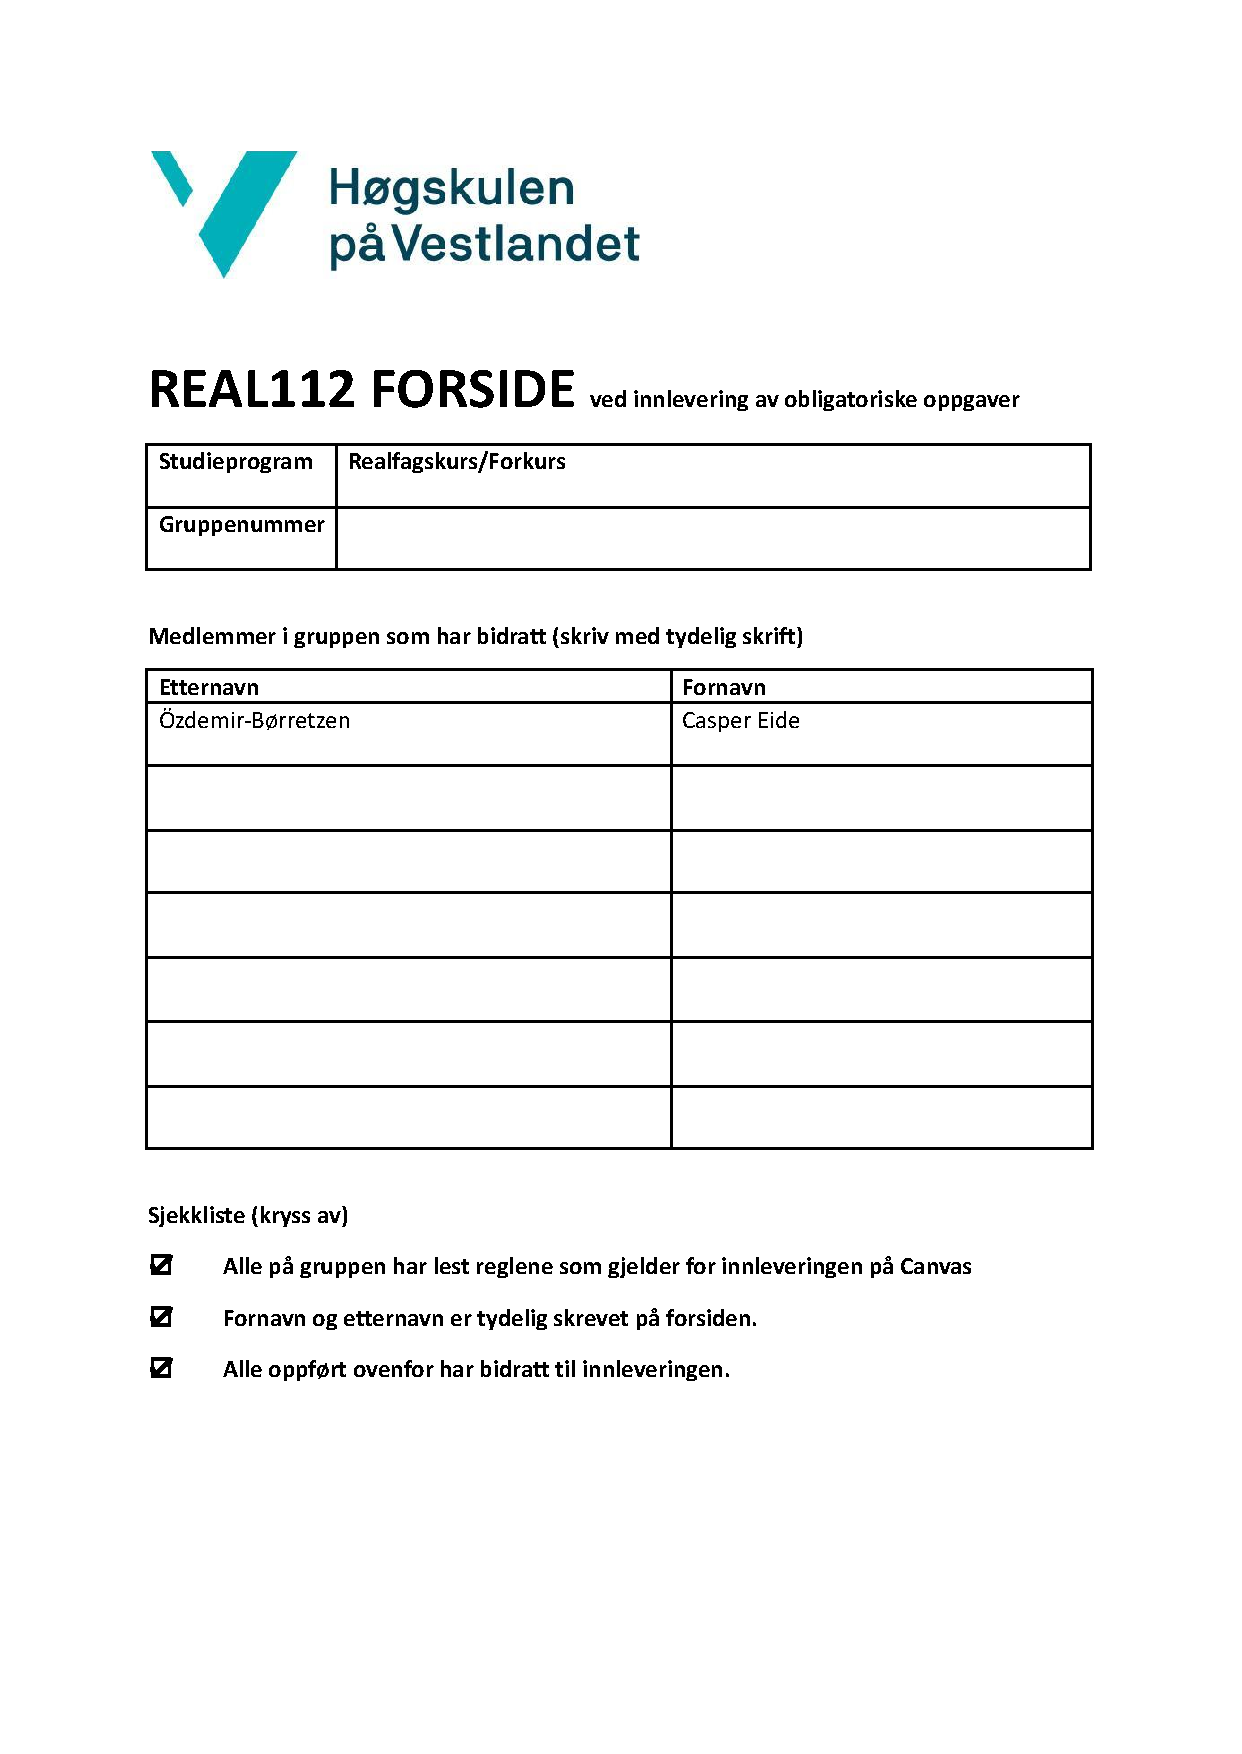
\includepdf[pages={1}]{real112-forside.pdf}

% % % % % % % % % % % % % % % % % % % % % % % % % % % % % % % % % % % % % % % % 

\opg{1}
\begin{enumerate}[leftmargin=*,itemsep=1cm,labelsep=2em,label=\alph*)]
\item[]
\begin{align*}
f &\rightarrow (ii)\\
f' &\rightarrow (i)\\
f'' &\rightarrow (iii)
\end{align*}

Figur $(i)$ har et stigningstall som minsker mot null og alltid er positivt.\\
Figur $(ii)$ og $(iii)$ har stigningstall som alltid er positivt, og ettersom figurene har bunnpunkt ved $x=0$ har den deriverte av $(ii)$ og $(iii)$ nullpunkt ved $x=0$.\\
Den eneste figuren med nullpunkt i $x=0$ er $(i)$, så $(i)$ må være figuren til $f'$.\\
Figur $(i)$ er alltid økene, men veksten minsker mot null. Dette stemmer overens med stigningstallet til figur $(ii)$, og stigningstallet til figur $(i)$ stemmer overens med figur $(iii)$.\\
Så figur $(ii)$ er grafen til $f$ og figur $(iii)$ er grafen til $f''$.
\end{enumerate}

% % % % % % % % % % % % % % % % % % % % % % % % % % % % % % % % % % % % % % % % 

\opg{2}
\begin{enumerate}[leftmargin=*,itemsep=1cm,labelsep=2em,label=\alph*)]
\opgd{a}
\begin{align*}
\frac{1}{3} \cdot 3^{2x} &= 27 &&| \cdot 3\\
3^{2x} &= 81 && | \log \\
%\log 3^{2x} &= \log 81\\
x \m 2 \m \log 3 &= \log 81 &&| \div (2 \m \log 3)\\[0.1cm]
x &= \frac{\log 81}{2 \m \log 3}\\
\svaralign{x}{= 2}
\end{align*}

\opgd{b}
\begin{align*}
e^x - 5 + 6e^{-x} &= 0\\
e^x + \frac{6}{e^x} - 5 &= 0 && | \m e^x\\
(e^x)^2 + 6 - 5e^x &= 0\\
(e^x - 3)(e^x - 2) &= 0\\
e^x = 3 $\ \ eller\ \ $& e^x = 2\\
\svaralign{x = \ln 3 $\ \ eller\ \ $}{x = \ln 2}
\end{align*}

\opgd{c}
\begin{align*}
\ln (x + 1) + \ln (x - 1) &= 3 \ln 2\\
\ln (x + 1) + \ln (x - 1) &= \ln (2^3)\\
\ln (x + 1) + \ln (x - 1) &= \ln (8)\\
(x + 1) \m (x - 1) &= 8\\
x^2 - 1 &= 8\\
x &= \sqrt{9}\\
\svaralign{x}{= 3}
\end{align*}
\end{enumerate}

% % % % % % % % % % % % % % % % % % % % % % % % % % % % % % % % % % % % % % % % 

\opg{3}
\begin{enumerate}[leftmargin=*,itemsep=1cm,labelsep=2em,label=\alph*)]
\opgd{a}
\begin{align*}
f(x) &= 3e^{-\frac{1}{2}x^2+x}\\
f'(x) &= 3e^{-\frac{1}{2}x^2+x} \m \left( -\frac{1}{2}x^2+x \right)'\\
f'(x) &= 3e^{-\frac{1}{2}x^2+x} \m (-x + 1)\\
\svaralign{f'(x)}{= 3e^{-\frac{1}{2}x^2+x} - 3x \m e^{-\frac{1}{2}x^2+x}}
\end{align*}

\opgd{b}
\begin{align*}
g(x) &= 3x^3 \ln x\\
g'(x) &= (3x^3) \m (\ln x)' + (3x^3)' \m (\ln x)\\
g'(x) &= 3x^3 \m \frac{1}{x} + 9x^2 \m \ln x\\[0.1 cm]
g'(x) &= 9x^2 \m \ln x + \frac{3x^3}{x}\\[0.1 cm]
\svaralign{g'(x)}{= 9x^2 \m \ln x + 3x^2}
\end{align*}

\opgd{c}
\begin{align*}
h(x) = \frac{x}{e^5}\\[0.2 cm]
\uuline{h'(x) = \frac{1}{e^5}}
\end{align*}

\opgd{d}
\begin{align*}
y(x) &= (e^x + 1)^5\\
y'(x) &= (e^x + 1)' \m 5 \m (e^x + 1)^4\\
\svaralign{y'(x)}{= 5e^x \m (e^x + 1)^4}
\end{align*}
\end{enumerate}

\newpage

% % % % % % % % % % % % % % % % % % % % % % % % % % % % % % % % % % % % % % % % 

\opg{4}
\begin{enumerate}[leftmargin=*,itemsep=1cm,labelsep=2em,label=\alph*)]
\opgd{a}
\begin{align*}
f(t) &= 2,50 - 2,50 \m e^{-0,012 \m t}\\
f(15) &= 2,50 - 2,50 \m e^{-0,18}\\
f(15) &= 0,4118244715 \approx 0,412\\
f(t) &= 2,00\\
2,50 - 2,50 \m e^{-0,012 \m t} &= 2,00 &&| -2,50\\
-2,50 \m e^{-0,012 \m t} &= -0,5 &&| \div -2,50\\
e^{-0,012 \m t} &= 0,2 &&| \ln() \m -1\\
0,012 \m t &= -ln(0,2) &&| \div 0,012\\[0.2 cm]
t &= \frac{-ln(0,2)}{0,012} = 134,119826 \approx 134\\
\end{align*}

\uuline{Etter 15 sekunder er konsentrasjonen $0,412\ millimol/L$.}

\uuline{Det tar 134 sekunder før konsentrasjonen er $2,00\ millimol/L$.}

\opgd{b} \ \\
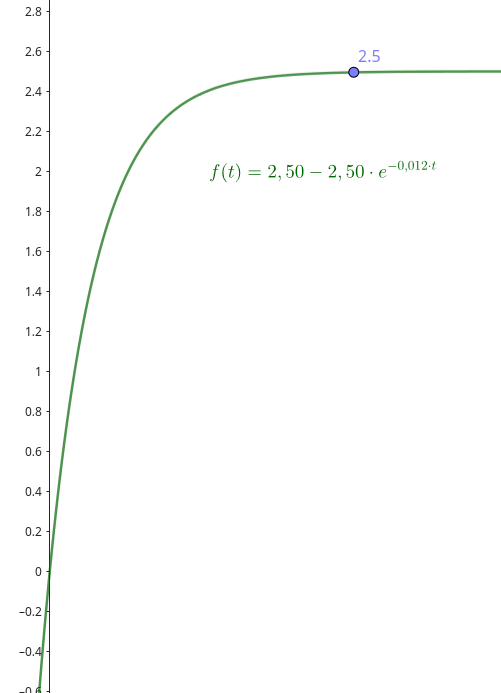
\includegraphics[scale=0.4]{4b.png}\\\\
\uuline{Konsentrasjonen vil etterhvert nærme seg $2,5\ millimol/L$.}

\opgd{c}
\begin{align*}
f'(t) &= -2,5 \m e^{-0,012 t} \m -0,012\\
f'(t) &= 0,03 \m e^{-0,012 t}\\
\svaralign{f'(134)}{= 0,03 \m e^{-1,608} = 0,0060086337 \approx 0,006}
\end{align*}

\end{enumerate}

% % % % % % % % % % % % % % % % % % % % % % % % % % % % % % % % % % % % % % % % 

\opg{5}
\begin{enumerate}[leftmargin=*,itemsep=1cm,labelsep=2em,label=\alph*)]
\opgd{a}
\begin{align*}
g(x) &= x-2 \ln (x^2 + 3),\ x \in \mathbb{R}\\
g'(x) &= (x)' - (2 \ln (x^2 + 3))' \m (x^2 + 3)\\
g'(x) &= 1 - 2 \m \frac{1}{x^2 + 3} \m 2x\\[0.2 cm]
g'(x) &= 1 - \frac{4x}{x^2 + 3}\\[0.2 cm]
g'(x) &= \frac{x^2 + 3}{x^2 + 3} - \frac{4x}{x^2 + 3}\\[0.2 cm]
g'(x) &= \uuline{\frac{x^2 - 4x + 3}{x^2 + 3}}
\end{align*}

\opgd{b}
\begin{align*}
g'(x) &= 0\\
x^2 - 4x + 3 &= 0\\
(x - 3) (x - 1) &= 0\\
x = 3 $\ \ eller\ \ $ &x = 1
\end{align*}

\begin{tikzpicture}[
negativ/.style={blue,dashed},
negativ_gray/.style={gray,dashed},
positiv/.style={blue},
positiv_gray/.style={gray},
vertlinje/.style={dotted,opacity=.7},
node distance=1.5ex,
nullpunkt/.style={fill=white,inner sep= 3pt}]
\draw [->,>=stealth] (-1,0) node (linestart) {} -- (7,0) node (lineend) {};
\node (null1) at (3,0) [label=above:3] {};
\node (null2) at (1,0) [label=above:1] {};
\node [matrix] (produktledd) [below left=of linestart]{
\node [left] (f1) {$(x-3)$}; \\
\node [left] (f2) {$(x-1)$}; \\
\node [left] (f3) {$g'(x)$}; \\
};
\draw [vertlinje] (null1)       -- (null1 |- f);
\draw [vertlinje] (null2)       -- (null2 |- f);
\draw [positiv_gray]   (null1 |- f1) -- (lineend |- f1);
\draw [negativ_gray]   (f1)          -- (null1 |- f1) node[nullpunkt] {$0$};
\draw [positiv_gray]   (null2 |- f2) -- (lineend |- f2);
\draw [negativ_gray]   (f2)          -- (null2 |- f2) node[nullpunkt] {$0$};
\draw [negativ]   (null2 |- f3) -- (null1 |- f3);
\draw [positiv]   (f3)          -- (null2 |- f3) node[nullpunkt] {$0$};
\draw [positiv]   (null1 |- f3) node[nullpunkt] {$0$} -- (lineend |- f3);
\end{tikzpicture}

\uuline{Grafen til $g$ har toppunkt ved $(1,\ g(1))$ og bunnpunkt ved $(3,\ g(3))$.}

\opgd{c}
\begin{align*}
g''(x) &= \frac{(x^2 - 4x + 3)' \m (x^2 + 3) - (x^2 - 4x + 3) \m (x^2 + 3)'}{(x^2 + 3)^2}\\[0.2 cm]
g''(x) &= \frac{ (2x - 4) (x^2 + 3) - (x^2 - 4x + 3) \m 2x }{(x^2 + 3)^2}\\[0.2 cm]
g''(x) &= \frac{ \cancel{2x^3} + \cancel{6x} - 4x^2 - 12 - \cancel{2x^3} + 8x^2 - \cancel{6x} }{ x^4 + 2 \m 3 \m x^2 + 3^2 }\\[0.2 cm]
g''(x) &= \frac{ 4x^2 - 12 }{ x^4 + 6x^2 + 9 }\\[0.4 cm]
g''(x) &= 0\\
4x^2 - 12 &= 0 &&| + 12\\
4x^2 &= 12 &&| \div 4\\
x^2 &= 3 &&| \sqrt{\ \ }\\
x &= \sqrt[\pm]{3}
\end{align*}

\uuline{Grafen til $g$ har vendepunkt ved $x$-koordinaten $\sqrt{3}$ og ved $-\sqrt{3}$.}

\end{enumerate}

% % % % % % % % % % % % % % % % % % % % % % % % % % % % % % % % % % % % % % % % 

\newpage
\opg{6}
\begin{enumerate}[leftmargin=*,itemsep=1cm,labelsep=2em,label=\alph*)]
\opgd{a}
\begin{align*}
\angle A &= 56 \degree\\
\angle ADB &= 80 \degree\\
\angle ABD &= 180 \degree - \angle A - \angle ADB = 44 \degree\\
\angle CDB &= 52 \degree\\
AB &= 60\ m\\
CD &= 50\ m
\end{align*}

\begin{align*}
BD &= \frac{AB}{\sin \angle ADB} \m \angle A = 50,50960881\ m \approx 51\ m\\\\
AD &= \frac{AB}{\sin \angle ADB} \m \angle ABD = 42,32247573\ m \approx 42\ m\\\\
BC &= \sqrt{BD^2 + CD^2 - 2 \m BD \m CD \m \cos \angle CDB} = 44,06289317 \approx 44\ m
\end{align*}

\begin{center}\uuline{$AD$ er $42\ m$, $BD$ er $51\ m$ og $BC$ er $44\ m$.}\end{center}

\opgd{b}
\begin{align*}
\frac{1}{2} \m BD \m CD \m \sin \angle CDB + \frac{1}{2} \m AD \m AB \m \sin \angle A = 2047,660549\ m^2 \approx 2048\ m^2
\end{align*}

\begin{center}\uuline{Arealet av tomten er $2048\ m^2$.}\end{center}

\end{enumerate}

% % % % % % % % % % % % % % % % % % % % % % % % % % % % % % % % % % % % % % % % 

\opg{7}
\begin{enumerate}[leftmargin=*,itemsep=1cm,labelsep=2em,label=\alph*)]
\item[]
\lstinputlisting[language=Python]{opg7.py}
\end{enumerate}

\end{document}
